\section{Auswertung}
\label{sec:Auswertung}
Für die Auswertung werden die folgende Größen benötigt.
\begin{align*}
  &\text{spezifische Wärmekapazität}\, Cp=75.38(\si{\frac{\joule}{\mol\kelvin}})  \\
  &\text{Dichte Wasser}\, 55.389\si{\frac{\mol}{\liter}} (294.85 \si{\kelvin,1\bar)}     \\
  &\text{molare Masse von} \, Cl_2F_2C \, (120,9135 \si{\frac{\gram}{\mol}})       \\
  &p_0=1       \si{\frac{\kilo\gram}{\meter^2}}      \\
  &\rho_0=5.51  \si{\frac{\kilo\gram}{\meter^3}}     \\
  &T_0=273.15  \si{\kelvin}                          \\
  &m_2c_w=12525.66845 \si{\frac{\joule}{\kelvin}}    \\
  &m_kc_k=660   \si{\frac{\joule}{\kelvin}}
\end{align*}
In der folgenden Tabelle sind alle Messwerte aufgeführt.
\begin{table}
  \centering
  \begin{tabular}{c c c c c c}
    \toprule
    Zeit/min & $T_1/\si{\kelvin}$ & $T_2/\si{\kelvin}$ & $p_a/\si{\bar}$ & $p_b/\si{\bar}$ & $N/\si{\watt}$ \\
    \midrule
    0 & 294.8\pm0.1 & 295.0\pm0.1 &  5.1\pm0.1 &  5.2\pm0.1  & 170\pm5 \\
    1 & 295.2\pm0.1 & 294.9\pm0.1 &  2.4\pm0.1 &  7.0\pm0.1  & 170\pm5 \\
    2 & 296.4\pm0.1 & 294.9\pm0.1 &  2.8\pm0.1 &  7.2\pm0.1  & 180\pm5 \\
    3 & 297.7\pm0.1 & 294.0\pm0.1 &  3.0\pm0.1 &  7.7\pm0.1  & 190\pm5 \\
    4 & 299.3\pm0.1 & 292.5\pm0.1 &  3.1\pm0.1 &  8.2\pm0.1  & 195\pm5 \\
    5 & 301.1\pm0.1 & 290.7\pm0.1 &  3.1\pm0.1 &  8.3\pm0.1  & 200\pm5 \\
    6 & 303.0\pm0.1 & 288.9\pm0.1 &  3.1\pm0.1 &  9.0\pm0.1  & 200\pm5 \\
    7 & 305.1\pm0.1 & 287.2\pm0.1 &  3.1\pm0.1 & 10.0\pm0.1  & 205\pm5 \\
    8 & 308.2\pm0.1 & 285.4\pm0.1 &  3.1\pm0.1 & 10.5\pm0.1  & 205\pm5 \\
    9 & 310.6\pm0.1 & 283.8\pm0.1 &  3.1\pm0.1 & 10.9\pm0.1  & 208\pm5 \\
   10 & 310.0\pm0.1 & 282.1\pm0.1 &  3.1\pm0.1 & 10.4\pm0.1  & 210\pm5 \\
   11 & 311.9\pm0.1 & 280.5\pm0.1 &  3.1\pm0.1 & 11.7\pm0.1  & 208\pm5 \\
   12 & 313.5\pm0.1 & 279.1\pm0.1 &  3.1\pm0.1 & 11.0\pm0.1  & 208\pm5 \\
   13 & 315.2\pm0.1 & 277.5\pm0.1 &  3.1\pm0.1 & 11.4\pm0.1  & 210\pm5 \\
   14 & 316.7\pm0.1 & 276.1\pm0.1 &  3.1\pm0.1 & 11.9\pm0.1  & 210\pm5 \\
   15 & 318.3\pm0.1 & 274.7\pm0.1 &  3.2\pm0.1 & 12.0\pm0.1  & 210\pm5 \\
   16 & 319.8\pm0.1 & 273.6\pm0.1 &  3.2\pm0.1 & 12.5\pm0.1  & 210\pm5 \\
   17 & 321.1\pm0.1 & 272.8\pm0.1 &  3.2\pm0.1 & 13.0\pm0.1  & 210\pm5 \\
   18 & 322.6\pm0.1 & 272.4\pm0.1 &  3.2\pm0.1 & 13.1\pm0.1  & 210\pm5 \\
   19 & 323.8\pm0.1 & 272.1\pm0.1 &  3.2\pm0.1 & 13.5\pm0.1  & 210\pm5 \\
   \bottomrule
  \end{tabular}
  \caption{Messdatentabelle.}
  \label{tab:Data}
\end{table}

Die Temperaturverläufe sind in dem folgenden Diagramm dargestellt und mit einer
Ausgleichsrechnung approximiert.
\subsection{Temperaturausgleichskurve}
\begin{figure}
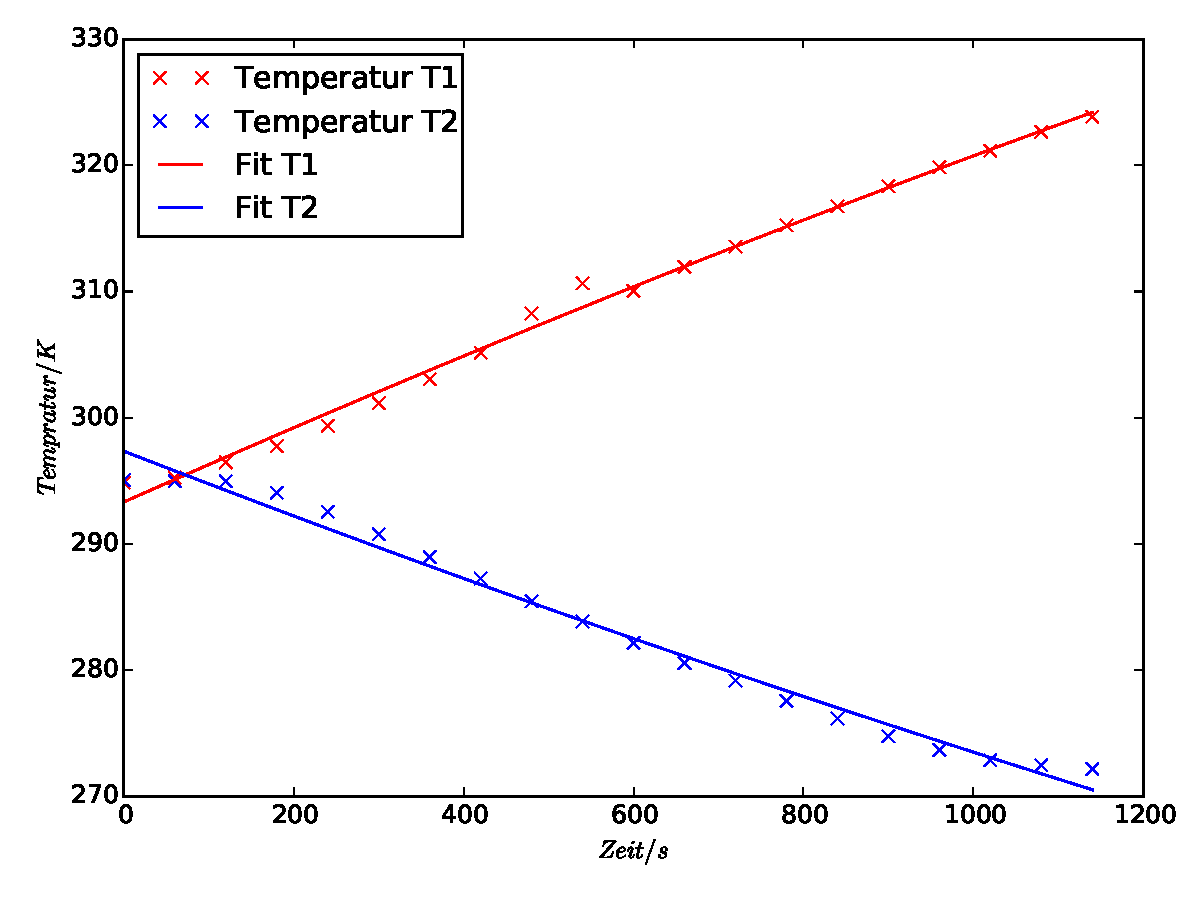
\includegraphics[height=13cm]{Temperaturgraphik.pdf}
\caption{Temperaturausgleichskurve.}
\end{figure}

Die Näherung entsteht mit scientific Python und ist gegeben durch
\begin{equation}
  T(t)=At^2+Bt+C .
\end{equation}
Die Parameter für erwärmte Reservoir $T_1$ sind

  $A=(-2.4857\cdot10^{-6}\pm1.6839\cdot10^{-6})\si{\frac{\kelvin}{\second^2}} $

  $B=(2.99251681\cdot10^{-2}\pm1.9886040\cdot10^{-3})\si{\frac{\kelvin}{\second}}$

  $C=(2.933127930141\cdot10^{2}\pm4.890916772\cdot10^{-1})\si{\kelvin}$

Die Parameter für den anderen Behälter $T_2$ sind

  $A=(2.2594\cdot10^{-6}\pm2.1868\cdot10^{-6})\si{\frac{\kelvin}{\second^2}}$

  $B=(-2.6112098\cdot10^{-2}\pm2.5825637\cdot10^{-3})\si{\frac{\kelvin}{\second}}$

  $C=(2.973393505497\cdot10^{2}\pm6.351744996\cdot10^{-1})\si{\kelvin}$

Die dazugehörigen Differentialquotienten erhält man durch die folgende Gleichung
\begin{equation}
\frac{dT}{dt}=2At+B
\end{equation}

\begin{table}
  \centering
  \begin{tabular}{c c c c c}
    \toprule
    $Zeit/s$ & $dT_1 /dt$ & Fehler & $dT_2 /dt$ &Fehler \\
    \midrule
    300  &  0.02843  &  \pm0.002230  & -0.02475  &  \pm0.002896  \\
    600  &  0.02694  &  \pm0.002835  & -0.02340  &  \pm0.003681  \\
    900  &  0.02545  &  \pm0.003625  & -0.02204  &  \pm0.004707  \\
   1140  &  0.02425  &  \pm0.004323  & -0.02096  &  \pm0.005615  \\
   \bottomrule
 \end{tabular}
 \caption{Differentialquotienten.}
 \label{tab:Diffquo}
\end{table}
\subsection{Güteziffer}
Als nächstes soll die Güteziffer bestimmt werden. Dafür nutzt man die Gleichung
\eqref{eqn:gueteziffer_ideal} für die ideale Güteziffer und die Gleichung
\eqref{eqn:berechnung_gueteziffer}
\begin{table}
  \centering

  \begin{tabular}{c c c c c}
    \toprule
    $Zeit/s$ & $v_\symup{ideal}$ &  Fehler  &  $v_\symup{real}$  &  Fehler\\
    \midrule
      300  &  28.956730  &  \pm0.3870202  &  1.874590  &  \pm0.154343  \\
      600  &  11.112903  &  \pm0.0538550  &  1.691679  &  \pm0.182511  \\
      900  &  7.3016055  &  \pm0.0221212  &  1.598035  &  \pm0.230776  \\
     1140  &  6.2640232  &  \pm0.0158262  &  1.523119  &  \pm0.273894  \\
   \bottomrule
 \end{tabular}
 \caption{Güteziffer}
 \label{tab:Gütez}
\end{table}
\subsection{Massendurchsatz}
Für den Massendurchsatz wird die Verdampfungswärme $L=(2.341\pm0.021)\cdot10^{4}$
benötigt. Diese errechnet sich der Steigung einer Approximation der
Dampfdruckkurvenwertepaare.
\begin{figure}
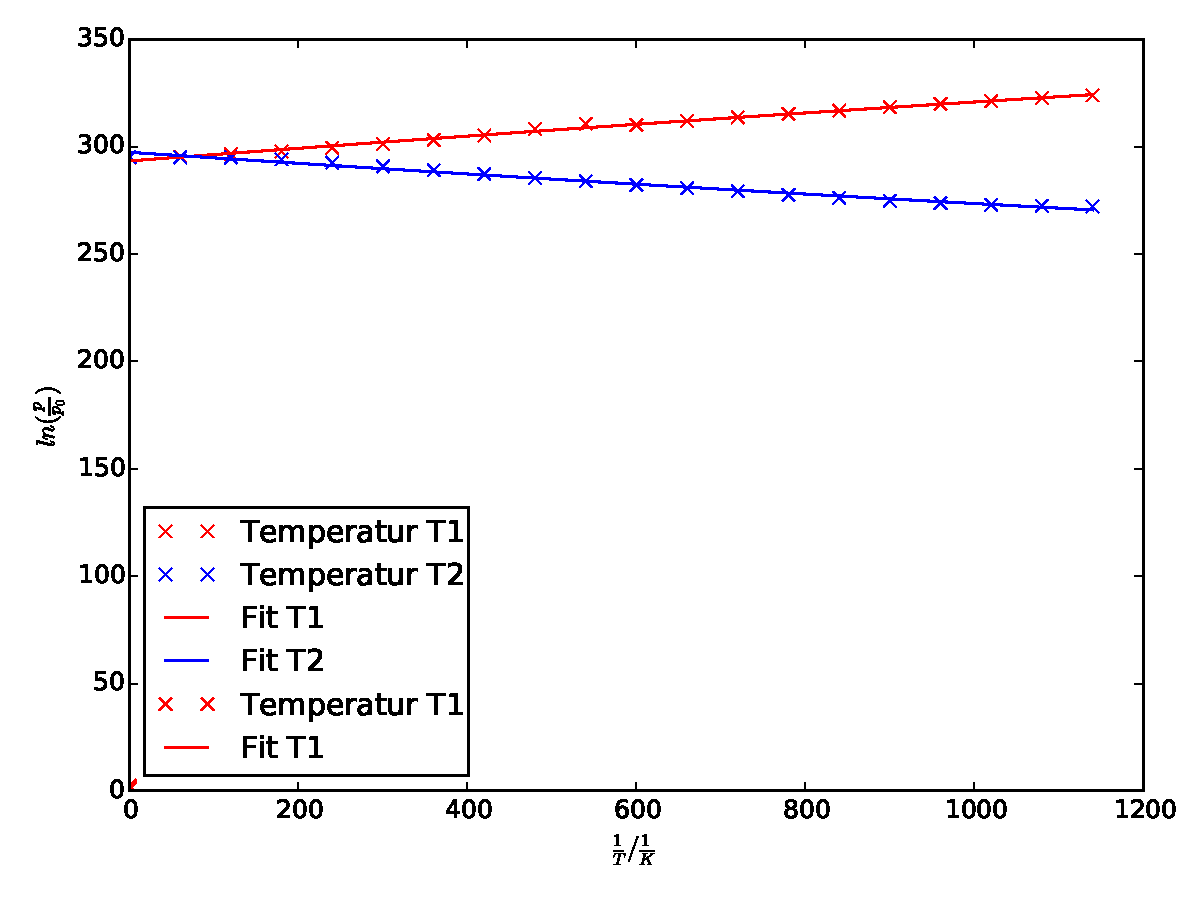
\includegraphics[height=13cm]{prog/daten/Dampfdruckkurve.pdf}
\caption{Verdampfungswärme.}
\end{figure}
Wenn die Werte in Gleichung \eqref{eqn:massendurchsatz}
einsetzt werden, ergibt sich der Massendurchsatz.

\begin{table}
  \centering
\begin{tabular}{c c c c c c c}
  \toprule
  $Zeit /s$ & $\frac{dQ_2}{dt}/\si{\joule}$ &  Fehler  & $\frac{dm}{dt}/\si{\frac{\mol}{\second}}$
   & Fehler  &  $\frac{dm}{dt} /\si{\frac{\gram}{\second}}$  & Fehler\\
  \midrule
  300  &   -326.43016  &  \pm38.19584  & 0.01394  &  \pm0.001636  &  1.68629  &  \pm0.19790  \\
  600  &   -308.55485  &  \pm48.54797  & 0.01318  &  \pm0.002077  &  1.59395  &  \pm0.25120  \\
  900  &   -290.67955  &  \pm62.07691  & 0.01241  &  \pm0.002654  &  1.50161  &  \pm0.32097  \\
 1140  &   -276.37931  &  \pm74.03976  & 0.01180  &  \pm0.003165  &  1.42774  &  \pm0.38269  \\
 \bottomrule
\end{tabular}
\caption{Massendurchsatz}
\label{tab:Massend}
\end{table}
\subsection{Mechanischekompressorleistung}
Die Dichte $\rho$, die für die Berechnung mechanischen Kompressorleistung
benötigt wird, kann berechnet werden, indem man die Gleichung der idealen Gase
umstellt.
\begin{equation}
  pV=nRT \leftrightarrow \frac{pV}{T}=nR
\end{equation}
Damit ergibt sich, da die Stoffmenge $n$ konstant bleibt,
\begin{equation}
  n_1=n_2
  \frac{p_0 V_0}{T_0}=\frac{p_2 V_2}{T_2}
\end{equation}
Da $ \rho V=m$ \leftrightarrow $V= \frac{m}{\rho}$ lässt sich \rho bestimmen wobei
$\rho_2=\rho$ und $p_2=p_a$.
\begin{equation}
  \rho=\frac{\rho_0 T_0 p_a}{T_2 p_0}
\end{equation}
Und mit Gleichung \eqref{eqn:kompressorleistung}
\begin{equation}
N_\symup{mech}=\frac{1}{\kappa-1}\left(p_b \sqrt[\kappa]{\frac{p_a}{p_b}}-p_a\right)\frac{1}{\frac{\rho_0 T_0 p_a}{T_2 p_0}}\frac{dm}{dt}
\end{equation}

\begin{table}
  \centering
\begin{tabular}{c c c c c}
  \toprule
  $Zeit /s$ & Dichte$\rho/\frac{g}{m^3}$ & Fehler & Leistung$N_\symup{mech} /W$  &  Fehler  \\
  \midrule
  300  &   15.49286  &  \pm0.49979  &  0.30985  &  \pm0.038141  \\
  600  &   15.04813  &  \pm0.48544  &  0.37588  &  \pm0.060299  \\
  900  &   15.12857  &  \pm0.47279  &  0.39983  &  \pm0.086119  \\
 1140  &   14.87164  &  \pm0.46476  &  0.42433  &  \pm0.114210  \\
 \bottomrule
\end{tabular}
\caption{Massendurchsatz}
\label{tab:Massend}
\end{table}
